\chapter{Arquitectura}

Para satisfacer los nuevos requerimientos que surgieron en esta nueva etapa, se tuvieron que hacer diferentes modificaciones a la arquitectura que se ten�a anteriormente. Estas modificaciones consistieron en su mayor�a en el agregado de nuevos componentes para realizar las nuevas funciones impuestas, y en menor medida, se amplio la funcionalidad de alguno de los m�dulos ya existentes. Si bien estas modificaciones no fueron grandes, tuvo una repercusi�n importante ya que el comportamiento del sistema cambio en gran medida.

Para solucionar el problema de las regiones y los gobiernos provinciales, se pens� la arquitectura para que contemple los nuevos requerimientos de la siguiente forma:

\begin{itemize}
\item Dentro de una regi�n, pueden existir varias provincias, por ende varios gobiernos provinciales.

\item Cada provincia, tiene una $Estacion$ $Central$ que toma y procesa los datos de la misma.

\item Los modelos pertenecientes a los gobiernos provinciales, podr�n procesar los datos de las Tr's dentro de su regi�n pero deber�n suscribirse a estaciones centrales de otras regiones en caso de necesitar datos que son sensadas por estas �ltimas.
\item Finalmente cualquier estaci�n central podr� comunicarse con otra para solicitar resultados parciales de acuerdo a su conveniencia.
\end{itemize}

\begin{figure}[h]
\centering
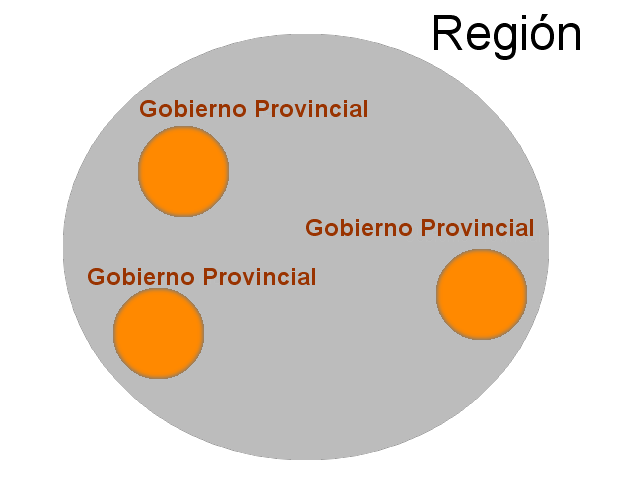
\includegraphics[scale=0.4]{regionProvincia.png}
\end{figure}

De �sta forma, se tiene un mejor control de los datos y los modelos de las diferentes provincias, ademas de distribuir la ejecuci�n de una misma regi�n.

La comunicaci�n entre $Estaciones$ $Centrales$ pude realizarse por diferentes medios de comunicaci�n, ya sea por gsm o por internet por ejemplo y eso estar� descripto en la descripci�n de funcionalidad del componente responsable de esa comunicaci�n. Esta comunicaci�n se realizar� mediante mensajes de control que permitan a una Estaci�n central, pedir resultados parciales de un modelo, o pedir informaci�n de ciertos sensores a otras Estaciones Centrales regionales.